\documentclass[notes, xcolor = dvipsnames]{beamer}

\usetheme{Warsaw}

\usepackage{amsmath}
\usepackage{graphicx}

\title{Memory Barriers: A Hardware view for Software Hackers}
\subtitle{Paul E. McKenney}

\author{Presented by \\ Akshay Gopalakrishnan}

\begin{document}
  
    \begin{frame}
        
        \maketitle
    \end{frame}


    \begin{frame}{Introduction}
        
        \begin{itemize}
            \item This paper represents the inner working of hardware that results in several non-sequential behaviors of our concurrent programs
            \item The paper is rife with examples as well as showcasing the reasons for having such hardware features which in turn help in our programs performing better.
            \item Along with the positives the author also carefully cautions why such rampant changes for performance might result in highly non-trivial behaviors being showcased by the hardware running our programs.
            \item The paper concludes by discussing the then versions of several concurrent hardware that exhibit different non-sequential behaviors.
        \end{itemize}

    \end{frame}

    \begin{frame}{Cache structures}
        
        \begin{figure}
            \makebox[\textwidth][c]{
                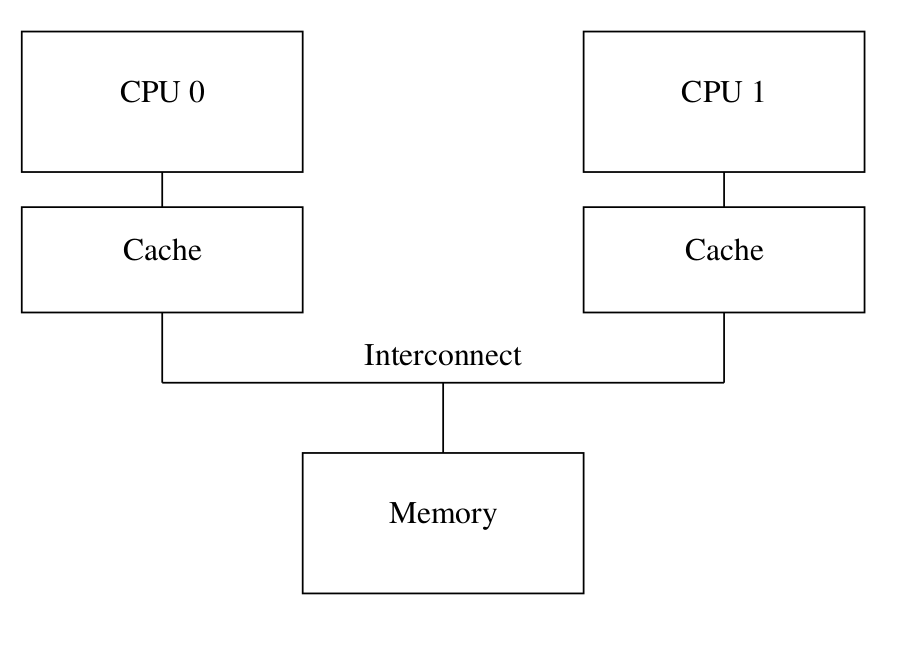
\includegraphics[scale=0.18]{CacheStructure.png}
            }
        \end{figure}

        \begin{itemize}
            \item An extra chunk of memory local to a given cpu (or multiple cpus in bigger systems).
            \item Data read from memory will also be saved in the cache if there is space. 
            \item Any subsequent accesses to the same memory will be first looked at in the cache and if not present, from the main memory.
        \end{itemize}

    \end{frame}

    \begin{frame}{The usefullness of Caches}
        
        \begin{itemize}
            \item Used for faster access of memory. 
            \item Useful when a single shared memory location is being accessed several times but not changed. 
            \item Need to read from main memory which is at least 10x times slower than accessing caches.
            \item Overall performance of program is significantly improved. 
        \end{itemize}

    \end{frame}

    \note{
        In modern systems there are multiple cache levels that exist, each of which is based on the scope. 
        For instance, L1 cache is local to just one core. Whereas L2 is to multiple cores in the same processor (could also be others). 
        All this layering is done for performance, part of the reason why we have such highly non-trivial behaviors of our concurrent programs.
    }

    \begin{frame}{THe MESI protocol}
        
        \begin{itemize}
            \item Multiple caches need to be in synchronization to ensure no stale data in caches exist. 
            \item Caches can communicate with each other via the interconnect network.
            \item We require a protocol to ensure that caches lines are updated accordingly. 
        \end{itemize}

        An example of such a protocol is MESI (Modified Exclusive Shared and Invalid).
        \begin{itemize}
            \item Modified - cache line has the upto date data which resides in memory and the data has been stored by the corresponding CPU. 
            \item Exclusive - cache line is not updated with the recent memory store done by the corresponding CPU. 
            \item Shared  - cache line is in read-only state (CPU needs to consult with other CPU caches before being able to write to it)
            \item Invalid - "empty" cache line and new data can be put here. 
        \end{itemize}


    \end{frame}

    \note{
        Modified state is when my CPU is writiing to memory some data as well as duly updated the cache line. Now this line has the only copy of the latest data in memory. 
        Exlcusive is one step behind modified state, wherein the CPU has updated memory, but not just its cache line. 
        Shared state is when more than one cache line has the same data of memory. This only means, if I want to change one cache line, I must inform the others too. 
        Invalid state can contain any stale data that is never going to be read by the CPU (as it is stale).
    }

    \begin{frame}{MESI Protocol Messages}

        The following messages are passed by a cache line to other caches in the system. 
        \begin{itemize}
            \item Read - Contains the physical address of the cache line to be read. 
            \item Read Response - Contains the data requested by a previous Read message.
            \item Invalidate - Contains the physical address of the cache line to be invalidated. 
            \item Invalidate Acknowledge - CPU receiving an Invalidate message must respond with this message once the specfied cache line is invalidated.
            \item Read Invalidate - Does the action of both Read and Invalidate in one message. 
            \item Writeback - Contains both the address and the data tobe written back to memory (could also implicitly update other cache lines with this).
        \end{itemize}
        
    \end{frame}

    \begin{frame}{Example of Cache Communication}

        The following table represents a sequence of actions done by CPU and the different states (MESI) of the caches after the action has been done. 
        \begin{figure}
            \makebox[\textwidth][c]{
                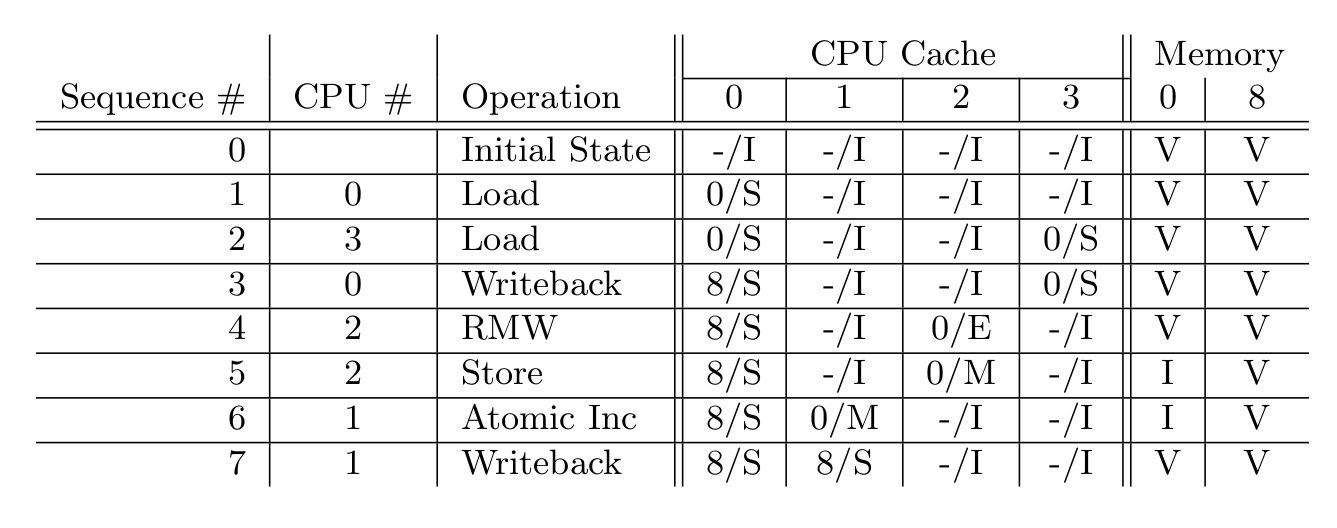
\includegraphics[scale=0.2]{MESI_Example.png}
            }
        \end{figure}
        
    \end{frame}

    \begin{frame}{Sequence 0 to 2}

        \begin{itemize}
            \item The 0th sequence represents the default state of cache before being used. 
                Each cache line is set to "Invalid" state. 
            \item The 1st sequence represents a load done by CPU 0 to fetch data from address 0. 
                The content in stored in CPU0 cache and the state changes to "Shared".
            \item The 2nd sequences represents a load done by CPU 0 to fethc data from address 0.
                The content is stored in CPU1 cache and the state changes to "Shared".
        \end{itemize}
        
    \end{frame}

    \begin{frame}{Sequence 3 to 5}

        \begin{itemize}
            \item The 3rd sequence represents a load done by CPU 0 to fetch data from address 8.
                This implicity means to Invalidate one's own cache line by sending an invalidate message to it. 
                This gives space to store data from address 0, which now is in the "Shared" state.
            \item The 4th sequence represents an RMW done by CPU 2 on address 0.
                Before it can do this, it needs to invalidate other caches having data on this address by sending "Invalidate" message.
                Once that is done, it's own cache (CPU 2) is set to "Exclusive" state, while others which had data at address 0 to "Invalid".
            \item The 5th sequence represents the actual store done by CPU 2 (as part of RMW).
                This changes its own cache to state "Modified" and sets the memory of address 0 to "Invalid".
        \end{itemize}
        
    \end{frame}

    \begin{frame}{Sequence 6 and 7}

        \begin{itemize}
            \item The 6th sequence represents CPU 1 performing an atomic write to data at Address 0.
                Since CPU 2 has its cache in modified state, the increment needs to change that value, while also invalidating their cache. 
                So a "Read Invalidate" message is sent to each cache line, get the updated store value and increment it by 1.
                Now it sets its own cache line (CPU 1) to modified state. 
                While other caches having data at address 0 is set ot invalidate. 
            \item The 7th sequence represents the actual commiting of the new data to memory. 
                This can either be done by actually issuing a writeback or forcing the cache to make space for other address data (via a Load).
                Here, a Load is issued for address 0 by CPU 1, which forces a writeback to address 0.
                The value at memory address 0 is updated and the state becomes "Valid".
                Meanwhile the cache line of CPU 1 has a "Shared" state.
        \end{itemize}
        
    \end{frame}


    \begin{frame}{Another example}

        Consider the example where CPU 0 wants to write to memory whose data is on cache line of CPU 1. 
        This would require the following actions
        \begin{itemize}
            \item CPU 0 sends an Invalidate message to CPU 1.
            \item CPU 1 receives the message, sets the appropriate cache line to "Invalid" state.
            \item CPU 1 sends the Acknowledgement message along with the data on the cache line to CPU 0.
            \item CPU 0 receives the Acknowledgement and data.
            \item CPU 0 does the write to memory and updates its own cache. 
        \end{itemize}

    \end{frame}

    \begin{frame}{Unnecessary stalls due to Writes}

        Notice that in the example above, CPU 0 needs to stall itself until the Acknowledgement message is received from CPU 1.
        This is showcased in the figure below.

        \begin{figure}
            \makebox[\textwidth][c]{
                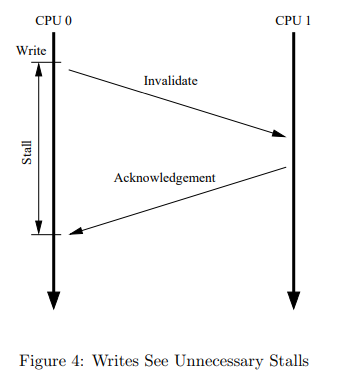
\includegraphics[scale=0.6]{Write_Stall.PNG}
            }
        \end{figure}

        CPU 0 need not stall as it will eventually do the write that it is supposed to do. 
        Rather it can continue doing some other task.

    \end{frame}

    \begin{frame}{Solution to write stalling: Write Buffers}
        
        One solution to this is to have a store buffer for each CPU.
        Writes to be done will be stored in this buffer and the CPU can continue doing future tasks.
        When the Acknowledgement messages are received by other CPUs, the write can be committed to its cache line (and eventually to memory).

        \begin{figure}
            \makebox[\textwidth][c]{
                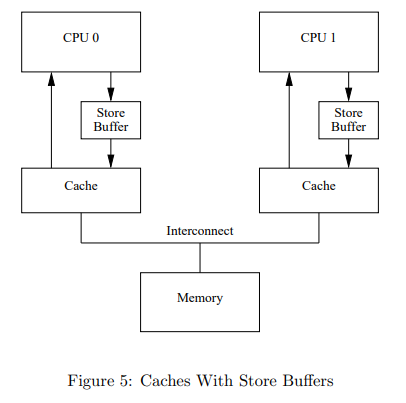
\includegraphics[scale=0.6]{WriteBuffers.PNG}
            }
        \end{figure}

    \end{frame}

    \begin{frame}{Added Complications}
        
        Adopting the above system does create its own problems. 
        \begin{itemize}
            \item The main cause is that writes to memory committed to store buffers are not read by the same CPU from it.
            \item Instead, the same memory is read either from cache or main memory.
            \item This means, the CPU uses a stale value of memory which results in incorrect execution of programs. 
        \end{itemize}

        \begin{figure}
            \makebox[\textwidth][c]{
                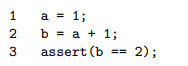
\includegraphics[scale=0.8]{WriteBufferProblem.PNG}
            }
        \end{figure}

    \end{frame}

    \note{Here is the reason why the example above fails. Consider only CPU 0 and 1 exist.
        \begin{itemize}
            \item CPU 0 wants to do the write $a=1$. So it sends a Read Invalidate message to CPU 1 and commits the store to its Store buffer. 
            \item CPU 1 receives the message and sends the invalidate with the current value of $a$ from its cache. 
            \item CPU 0 meanwhile wants to do $b = a + $, so starts reading $a$ from its own cache line. It receives the value 0. 
            \item Now CPU 0 receives the message from CPU 1 and the store buffer flushes the write to CPU 0 cache line. 
            \item CPU 0 does $b = a + 1$ having read $a=0$ from its cache before.
            \item Now $b=1$.
            \item The assertion fails.
        \end{itemize}
    }
    
    \begin{frame}{Solution seems simple: but?}
        
        The straightforward solution to this is to first let CPUs check their own store buffers during loads from memory and then if not found checking cache and/or memory. 
        However, this also does not prevent all our problems. 
        Consider the code below, where CPU 0 holds exclusive rights to cache line for $b$. 
        \begin{figure}
            \makebox[\textwidth][c]{
                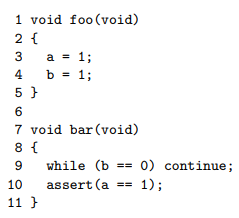
\includegraphics[scale=0.8]{WriteBufferProblem2.PNG}
            }
        \end{figure}
        The problem is that CPU 0 (if running the first code snippet) can upadte value of $b$ before committing the value of $a$ to cache.
        This may result in the assertion to fail.
    \end{frame}

    \note{
        The reason why this would happen is the following steps
        \begin{itemize}
            \item CPU 0 wants to do $a=1$, but $a$'s cache line is not exclusive/modified, so it sends the write to store buffer and sends Read Invalidate to CPU 1. 
            \item CPU 1 wants to do $while(b==0)$ so tries to read value of $b$. It does not exist in its cache line, so sends a read to CPU 0.  
            \item CPU 0 now wants to do $b=1$ and since it owns this cache line, commits the write immedidately to cache. 
            \item CPU 0 receives the read message from CPU 1 and sends $b=1$ as a response to CPU 1. 
            \end{itemize}
    }

    \note{

        \begin{itemize}
            \item CPU 1 receives the read invalidate for $a$ and sends Acknowledgement along with the value of $a$ to CPU 0. 
            \item CPU 1 then receives the value of $b$. Ends the loop (as $b=1$) and moves to assertion.
            \item The assertion fails. 
            \item CPU 0 receives the Acknowledgement from CPU 1 on $a$. So now it commits from store buffer to cache line.
        \end{itemize}

    }

    
    \begin{frame}{Here comes Write Memory Barriers}

        The problem now is that the hardware does not recognize dependencies between memory accesses (meaning things like conditionals and assertions like the above example).
        At this point, the hardware itself cannot do much.
        
        The solution to this was to have an instruction which specifically tells the hardware that some dependency exists.
        This instruction is called a Write Memory Barrier. 
        The following code with a write barrier solves our issue. 
        \begin{figure}
            \makebox[\textwidth][c]{
                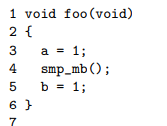
\includegraphics[scale=0.8]{WriteBarrierSol.PNG}
            }
        \end{figure}
        
    \end{frame}

    \note{
        The reason inserting a write memory barrier there solves our problem is that CPU 0 will never do the wrtie $b=1$ until the store buffer holding $a=1$ is first committed to cache. 
    }

    \begin{frame}{Yay store buffers ! But ? }
        
        Store buffers are good for performance. 
        But in hardware, these buffers are quite small. 
        So if they get full or the CPU needs to process a write barrier instruction, it must wait until all the writes are flushed.
        This in turn depends on whether the CPU has received invalidate acknowledgement from all the CPUs in the hardware. 
        This may take time as other CPUs may be busy accessing main memory or other cache lines at the moment, which take a long time. 
        In addition, to send acknowledgement, the CPU must first access its cache and tag the appropriate cache line Invalid. 
        All this takes longer and this stalling becomes a bottleneck for performance. 

    \end{frame}

    \begin{frame}{Invalidate queues}
        
        One observation is that the CPU need not actually invalidate the cache line immediately before sending acknowledgement.
        The CPU only needs to do this if another message for the same cache line is requested. 

        For this, each CPU is equipped with its own invalidate queue. 
        Invalidate requests are stored in this queue, promising the CPU requesting the acknowledgement that it would be done eventually. 
        So the acknowledgement message is often sent immediately without modifying the cache line state. 

        \begin{figure}
            \makebox[\textwidth][c]{
                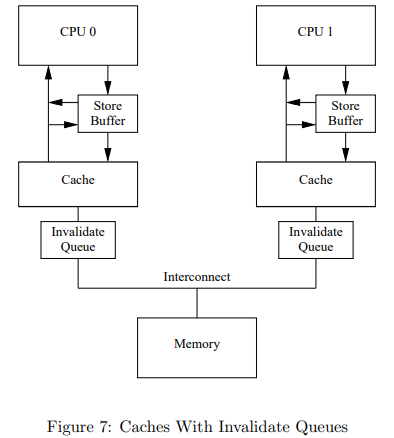
\includegraphics[scale=0.6]{InvalidateQueues.PNG}
            }
        \end{figure}

    \end{frame}

    \begin{frame}{Added Complications}
        
        While doing the above is good, the CPUs still are not concerned with the state of the cache if they themselves receive a read/write access to be performed.
        In essence, on a read, the CPU might end up reading a stale value from cache line (with the invalidate message for that line still in queue).

        The following example, run with store buffers and invalidate queues even with a write barrier will produce an incorrect result. 
        \begin{figure}
            \makebox[\textwidth][c]{
                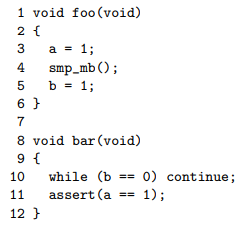
\includegraphics[scale=0.8]{InvalidateQueueProblem.PNG}
            }
        \end{figure}

    \end{frame}

    \note{
        The reason why the above example may lead to assertion failure is as follows. 
        Suppose CPU0 runs foo and CPU1 bar.
        Also suppose $a$ is in shared state in cache while CPU0 has exclusive rights to cache line of $b$. 
        \begin{itemize}
            \item CPU0 performs $a=1$. But the cache line is "Shared". So it sends an invalidate message to CPU1.
            \item CPU1 receives the message, immedidately sends acknowledgement. But CPU1 does not yet change the cache line of $a$ to "Invalid".
            \item CPU1 processes $while(b==0)$, by issuing a read request to CPU0 cache.
            \item CPU0 receives the acknowledgement. Now it updates its cache with the modified value of $a$. 
        \end{itemize}
    }

    \note{
        \begin{itemize}
            \item CPU0 processes the write barrier and proceeds to do $b=1$. Since it has exclusive right to it, updates the cache line of $b$ right away.
            \item Now CPU0 receives the read request for $b$ and sends the value $1$.
            \item CPU1 receives this value and ends the loop. 
            \item Now for the assertion, CPU1 reads the value of $a$ from its own cache (without processing hte invalidate message for it as it thinks nobody else it bothering it with another cache message for that line).
            \item Hence the assertion fails.
        \end{itemize}
    }

    \begin{frame}{Here comes Read Memory Barriers}
     
        The above example indicates that the memory barrier is sort of ignored. 
        One solution for this example is to ensure that when the CPU comes across a memory barrier, it ensures that its invalidate queue is serviced (emptied) before proceeding. 
        In literature one can say this as a read barrier. 
        So the solution to the above problem is a barrier that will be inserted in bar too.
        \begin{figure}
            \makebox[\textwidth][c]{
                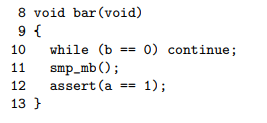
\includegraphics[scale=0.8]{ReadBarrierSolution.PNG}
            }
        \end{figure}
        
    \end{frame}

    \note{
        Currently, this is only viewed as a memory barrier instruction. 
        In many languages/hardwares, different variants of these barriers are provided. 
        Of these, we have looked at Read and Write barriers. 
        However, we can further dissect it based on what accesses should not occur before those accesses which precede the barrier. 
        Doing so, we get Read-Read(Read memory barrier), Read-Write, Write-Read and Write-Write(write memory barrier) variants of barriers.
    }

    \begin{frame}{Barrier instructions and their effect on ordering}

        While memory barriers are useful for ordering accesses, one has to note that they only order accesses for the CPU that performs these accesses. 
        This means, CPUs might observe incoming writes from other CPUs in different orders.
        This in literature is known as non-multicopy-atomicity. 
    
    \end{frame}

    \begin{frame}{Conclusion}
    
        \begin{itemize}
            \item Caches and buffers definitely help in performance improvements.
            \item However, this comes at a cost of non-trivial program behaviors.
            \item These behaviors can be controlled using barriers, but only upto some point. 
            \item The age-old tradeoff between performance and complexity in semantics to explain program execution can be seen firsthand here. 
            \item Perhaps we should not crave for so much performance?
            \item Perhaps just improve the cache coherence protocol system?  
        \end{itemize}

    \end{frame}

    \begin{frame}{Thank you!}
        
        Questions? 

    \end{frame}

\end{document}